\begin{center}
	\begin{tabular}{M{9.25cm}M{8.75cm}}
		\textbf{TRƯỜNG THCS-THPT NGUYỄN KHUYẾN}& \textbf{ÔN TẬP KIỂM TRA GIỮA HỌC KÌ II}\\
		\textbf{MÃ ĐỀ: 001}& \textbf{Bài thi môn: VẬT LÝ 10}\\
		\textit{(Đề thi có 03 trang)}& \textit{Thời gian làm bài: 45 phút, không kể phát đề}
		
		\noindent\rule{4cm}{0.8pt} \\
	\end{tabular}
\end{center}
\setcounter{section}{0}
\section{Câu trắc nghiệm nhiều phương án lựa chọn}
\textit{Thí sinh trả lời từ câu 1 đến câu 12. Mỗi câu hỏi thí sinh chọn một phương án}
\setcounter{ex}{0}
\Opensolutionfile{ans}[ans/D10-GK-HK2-001-TN]
% ===================================================================
\begin{ex}
	Phát biểu nào sau đây là \textbf{không đúng} khi nói về công của một lực?
	\choice
	{Công là đại lượng vô hướng}
	{\True Lực luôn sinh công khi điểm đặt của lực tác dụng lên vật dịch chuyển}
	{Trong nhiều trường hợp, công cản có thể có lợi}
	{Giá trị của công phụ thuộc vào góc hợp bởi vecto lực tác dụng và vecto độ dịch chuyển}
	\loigiai{}
\end{ex}

% ===================================================================
\begin{ex}
	Động năng của một vật \textbf{không} có đặc điểm nào sau đây?
	\choice
	{Phụ thuộc vào khối lượng của vật}
	{\True Không phụ thuộc vào hệ quy chiếu}
	{Là đại lượng vô hướng, không âm}
	{Phụ thuộc vào vận tốc của vật}
	\loigiai{}
\end{ex}

% ===================================================================
\begin{ex}
	Cơ năng của một vật bằng
	\choice
	{hiệu của động năng và thế năng của vật}
	{hiệu của thế năng và động năng của vật}
	{\True tổng động năng và thế năng của vật}
	{tích của động năng và thế năng của vật}
	\loigiai{}
\end{ex}

% ===================================================================
\begin{ex}
	Khi một quả bóng được ném lên thì
	\choice
	{\True động năng chuyển thành thế năng}
	{thế năng chuyển thành động năng}
	{động năng chuyển thành cơ năng}
	{cơ năng chuyển thành động năng}
	\loigiai{}
\end{ex}
% ===================================================================
\begin{ex}
	Động năng của vật sẽ thay đổi như thế nào nếu khối lượng của vật tăng gấp đôi và tốc độ của vật giảm còn một nửa?
	\choice
	{Không đổi}
	{\True Giảm 2 lần}
	{Tăng 2 lần}
	{Giảm 4 lần}
	\loigiai{}
\end{ex}
% ===================================================================
\begin{ex}
	 \immini{Ba quả bóng giống hệt nhau được ném ở cùng một độ cao từ đỉnh của toà nhà như hình bên. Quả bóng (1) được ném phương ngang, quả bóng (2) được ném xiên lên trên, quả bóng (3) được ném xiên xuống dưới. Các quả bóng được ném với cùng tốc độ đầu. Bỏ qua lực cản của không khí. Sắp xếp tốc độ của các quả bóng khi chạm đất theo thứ tự giảm dần.\choice
	 	{1, 2, 3}
	 	{2, 1, 3}
	 	{3, 1, 2}
	 	{\True Ba quả bóng chạm đất với cùng tốc độ}}
	 {\vspace{-0.5cm}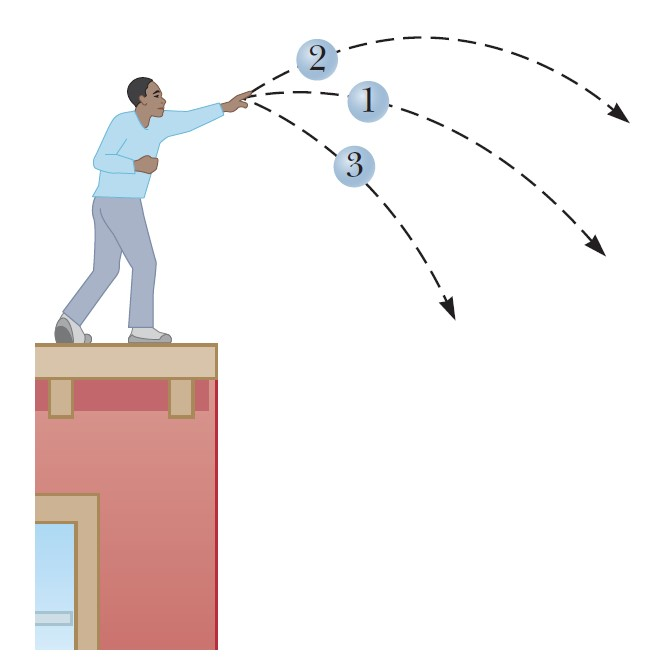
\includegraphics[scale=0.5]{../figs/D10-GK-HK2-1}}
	\loigiai{}
\end{ex}

% ===================================================================
\begin{ex}
	Đơn vị nào sau đây \textbf{không được dùng} để đo công suất?
	\choice
	{\SI{}{\watt}}
	{\True \SI{}{\joule \cdot \second}}
	{\si{HP}}
	{\SI{}{\kilogram \cdot \meter\squared / \second \cubed}}
	\loigiai{}
\end{ex}


% ===================================================================
\begin{ex}
	 Một vận động viên trượt tuyết có tổng khối lượng \SI{60}{\kilogram} bắt đầu trượt trên đồi tuyết từ điểm A đến điểm B. Biết điểm A có độ cao lớn hơn điểm B là \SI{10}{\meter}. Giả sử lực cản là không đáng kể. Lấy $g=\SI{10}{\meter/\second^2}$. Động năng của vận động viên này khi đến vị trí B là bao nhiêu?
	\choice
	{\True \SI{6E3}{\joule}}
	{\SI{3E2}{\joule}}
	{\SI{60}{\joule}}
	{Không xác định được vì còn phụ thuộc vào việc chọn gốc thế năng}
	\loigiai{}
\end{ex}
% ===================================================================
\begin{ex}
	Một vật được thả rơi tự do từ độ cao $h=\SI{60}{\meter}$ so với mặt đất. Vị trí mà vật có động năng gấp đôi thế năng cách mặt đất một đoạn
	\choice
	{\SI{40}{\meter}}
	{\SI{30}{\meter}}
	{\True \SI{20}{\meter}}
	{\SI{10}{\meter}}
	\loigiai{}
\end{ex}


% ===================================================================
\begin{ex}
	\immini{Thùng được kéo trượt theo phương ngang bằng lực $\vec{F}$ như hình bên. Nhận định nào sau đây về công của trọng lực $\vec{P}$ và phản lực $\vec{N}$ khi tác dụng lên thùng là đúng?
		}
	{\vspace{-0.5cm}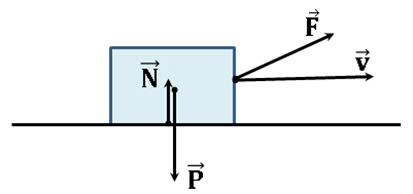
\includegraphics[scale=0.3]{../figs/LTTHPT-TOPIC3-12}}
	\choice
	{\( A_{\vec{N}} > A_{\vec{P}}\)}
	{\( A_{\vec{N}} < A_{\vec{P}}\)}
	{\True \( A_{\vec{N}} = A_{\vec{P}}=0\)}
	{\( A_{\vec{N}} = A_{\vec{P}}\neq 0\)}
	\loigiai{}
\end{ex}

% ===============% ===================================================================
\begin{ex}
	Một vật có khối lượng 1 tấn đang chuyển động với tốc độ \SI{72}{\kilo\meter/\hour} thì động năng của nó bằng
	\choice
	{\SI{7200}{\joule}}
	{\SI{200}{\joule}}
	{\True \SI{200}{\kilo\joule}}
	{\SI{72}{\kilo\joule}}
	\loigiai{}
\end{ex}

%====================================================
\begin{ex}
	Một vật khối lượng $\SI{2}{\kilogram}$ bị hất đi với vận tốc ban đầu có độ lớn $\SI{4}{\meter / \second}$ để trượt trên mặt phẳng nằm ngang. Sau khi trượt được $\SI{0.8}{\meter}$ thì vật dừng lại. Công của lực ma sát đã thực hiện bằng
	\choice
	{$\SI{2.5}{\joule}$}
	{\True $\SI{-16}{\joule}$}
	{$\SI{-2.5}{\joule}$}
	{$\SI{16}{\joule}$}
	\loigiai{}
\end{ex}
\Closesolutionfile{ans}
\section{Câu trắc nghiệm đúng/sai} 
\textit{Thí sinh trả lời từ câu 1 đến câu 4. Trong mỗi ý \textbf{a)}, \textbf{b)}, \textbf{c)}, \textbf{d)} ở mỗi câu, thí sinh chọn đúng hoặc sai}
\setcounter{ex}{0}\\
\Opensolutionfile{ans}[ans/D10-GK-HK2-001-TF]
% ===================================================================
\begin{ex}
	Chọn đúng/ sai cho các ý sau
	\choiceTF
	{\True Khi di chuyển xe lên dốc thì người lái xe sang số nhỏ để tăng lực kéo}
	{\True Đại lượng để so sánh khả năng thực hiện công của các máy móc khác nhau trong cùng một khoảng thời gian là công suất}
	{Giá trị của công không phụ thuộc vào hệ quy chiếu}
	{Công của lực bằng 0 khi lực hợp với phương chuyển động một góc $\SI{180}{\degree}$}
	\loigiai{
		\begin{enumerate}[label=\alph*)] %alph=> arabic nếu muốn sử dụng số
			\item Đúng.
			\item Đúng.
			\item Sai. Giá trị của công trong hệ quy chiếu quán tính và phi quán tính là khác nhau.
			\item Sai. Công cản, có giá trị âm.
		\end{enumerate}
	}
\end{ex}
% ===================================================================
\begin{ex}
	Hai anh công nhân dùng ròng rọc để kéo đều một xô vữa lên các tầng cao của một công trình xây dựng. Dựa vào bảng số liệu dưới đây, hãy xác định các phát biểu dưới đây đúng hay sai? Lấy $g=\SI{10}{\meter / \second \squared}$.
	\begin{center}
		\renewcommand{\arraystretch}{1.1} % Tăng khoảng cách dòng để dễ đọc hơn
		\setlength{\tabcolsep}{8pt} % Điều chỉnh khoảng cách giữa các cột
		\resizebox{0.95\textwidth}{!}{
			\begin{tabular}{|c|c|c|c|c|}
				\hline
				\textbf{Công nhân} & \textbf{Khối lượng xô vữa} & \textbf{Độ cao công trình} & \textbf{Công thực hiện} & \textbf{Thời gian thực hiện} \\
				& \( m \) ($\SI{}{\kilogram}$) & \( h \) ($\SI{}{\meter}$) & \( A \) ($\SI{}{\joule}$) & \( t \) ($\SI{}{\second}$) \\
				\hline
				Công nhân 1 & \( m_1 = 20 \) $\SI{}{\kilogram}$ & \( h_1 = 10 \) $\SI{}{\meter}$ & \( A_1 = \dots ? \dots \) & \( t_1 = 10 \) $\SI{}{\second}$ \\
				\hline
				Công nhân 2 & \( m_2 = 21 \) $\SI{}{\kilogram}$ & \( h_2 = 11 \) $\SI{}{\meter}$ & \( A_2 = \dots ? \dots \) & \( t_2 = 20 \) $\SI{}{\second}$ \\
				\hline
		\end{tabular}}
	\end{center}
	\choiceTF
	{\True Công suất của công nhân 1 là $\SI{200}{\watt}$}
	{Công suất của công nhân 2 là $\SI{500}{\watt}$}
	{\True Công nhân 1 thực hiện công nhanh hơn công nhân 2}
	{Nếu công nhân 2 thực hiện công việc của công nhân 1 thì thời gian thực hiện công việc là $\SI{19}{\second}$}
	\loigiai{
		\begin{enumerate}[label=\alph*)] %alph=> arabic nếu muốn sử dụng số
			\item Đúng. $P_1=\dfrac{m_1gh_1}{t_1}=\SI{200}{\watt}$
			\item Sai. $P_2=\dfrac{m_2gh_2}{t_2}=\SI{115.5}{\watt}$
			\item Đúng. Công suất của công nhân 1 lớn hơn công nhân 2
			\item Sai. $t_2'=\dfrac{m_1gh_1}{P_2}=\SI{17.3}{\second}$
		\end{enumerate}
	}
\end{ex}
% ===================================================================
\begin{ex}
	Một con châu chấu cơ bắp đã thực hiện một cú bật nhảy theo phương xiên góc \SI{45}{\degree} từ mặt đất như hình minh họa bên. Nó đạt độ cao tối đa \SI{1.00}{\meter} sau cú nhảy. Bỏ qua sức cản của không khí. Lấy $g=\SI{9.80}{\meter/\second^2}$.
	\immini{
		\choiceTF
		{\True Trong giai đoạn nhảy lên, tốc độ của con châu chấu giảm dần}
		{Tại vị trí có độ cao cực đại, tốc độ của con châu chấu bằng 0}
		{\True Tốc độ của châu chấu khi vừa bật khỏi đất là \SI{6.26}{\meter/\second}}
		{Vị trí chạm đất của châu chấu cách vị trí ban đầu đoạn khoảng \SI{5.66}{\meter}}}
	{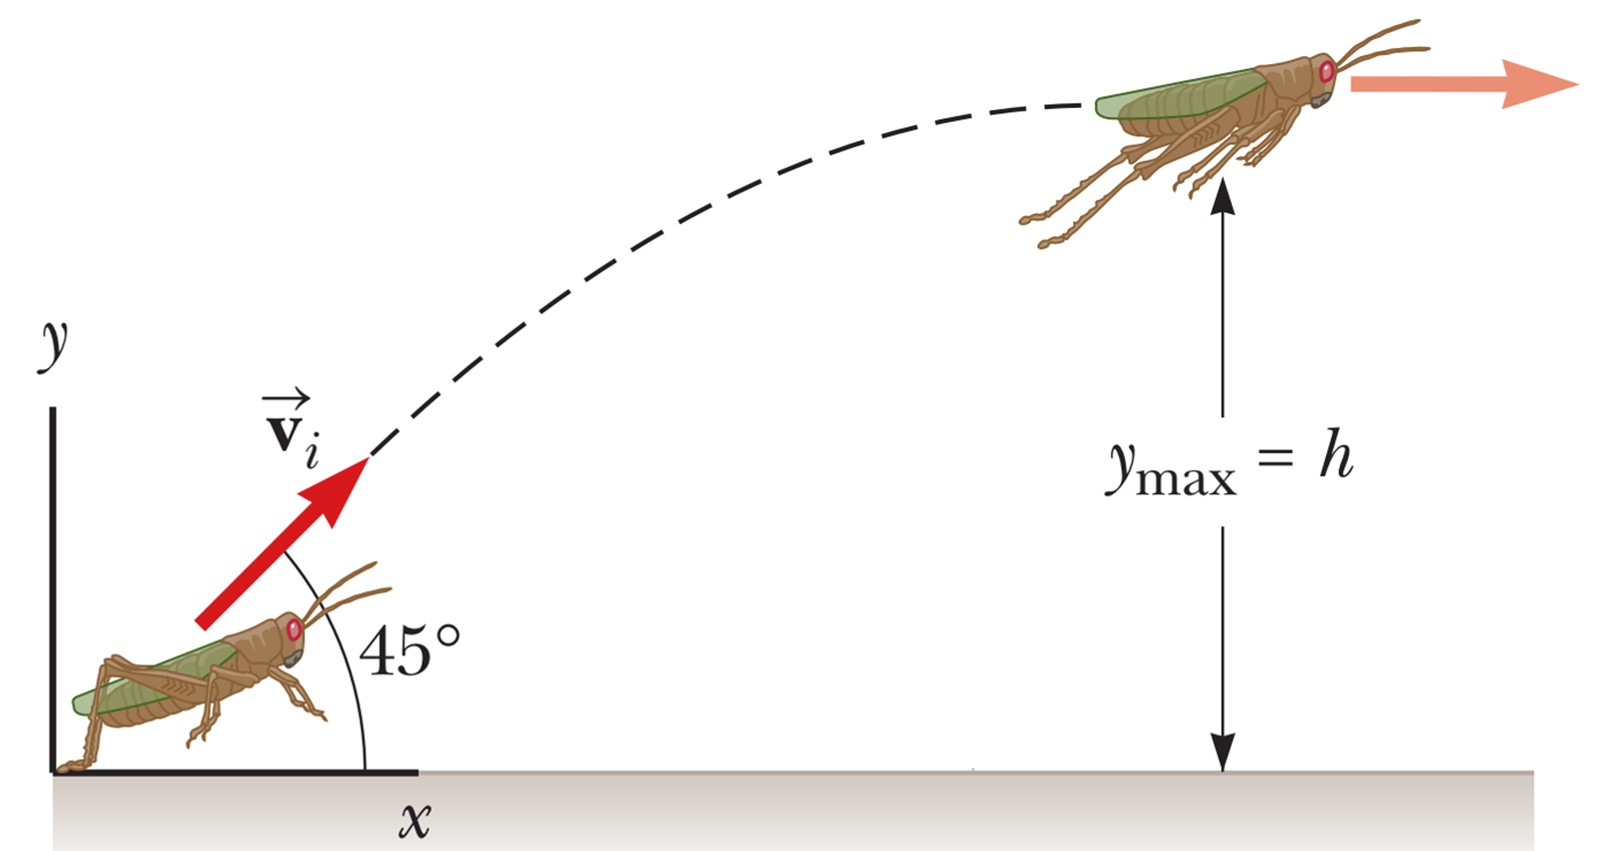
\includegraphics[scale=0.25]{../figs/D10-GK-HK2-3}}
	\loigiai{}
\end{ex}
% ===================================================================
\begin{ex}
	\immini{Một con lắc đơn gồm một quả cầu nặng $\SI{0.025}{\kilogram}$ treo vào đầu dây dài như hình. Kéo con lắc đến vị trí M rồi thả ra. Bỏ qua mọi lực cản, xem như dây không co dãn và khối lượng của sợi dây không đáng kể. Lấy $g=\SI{10}{\meter/\second^2}$. Chọn gốc thế năng tại vị trí thấp nhất của con lắc.
		\choiceTF
		{\True Trong quá trình chuyển động, cơ năng của con lắc được bảo toàn}
		{\True Thế năng của quả cầu tại vị trí M là $\SI{0.06}{\joule}$}
		{\True Khi quả cầu ở vị trí M thì thế năng của quả cầu cực đại}
		{\True Tốc độ quả cầu ở vị trí O gần bằng $\SI{2.19}{\meter/\second}$}
	}
	{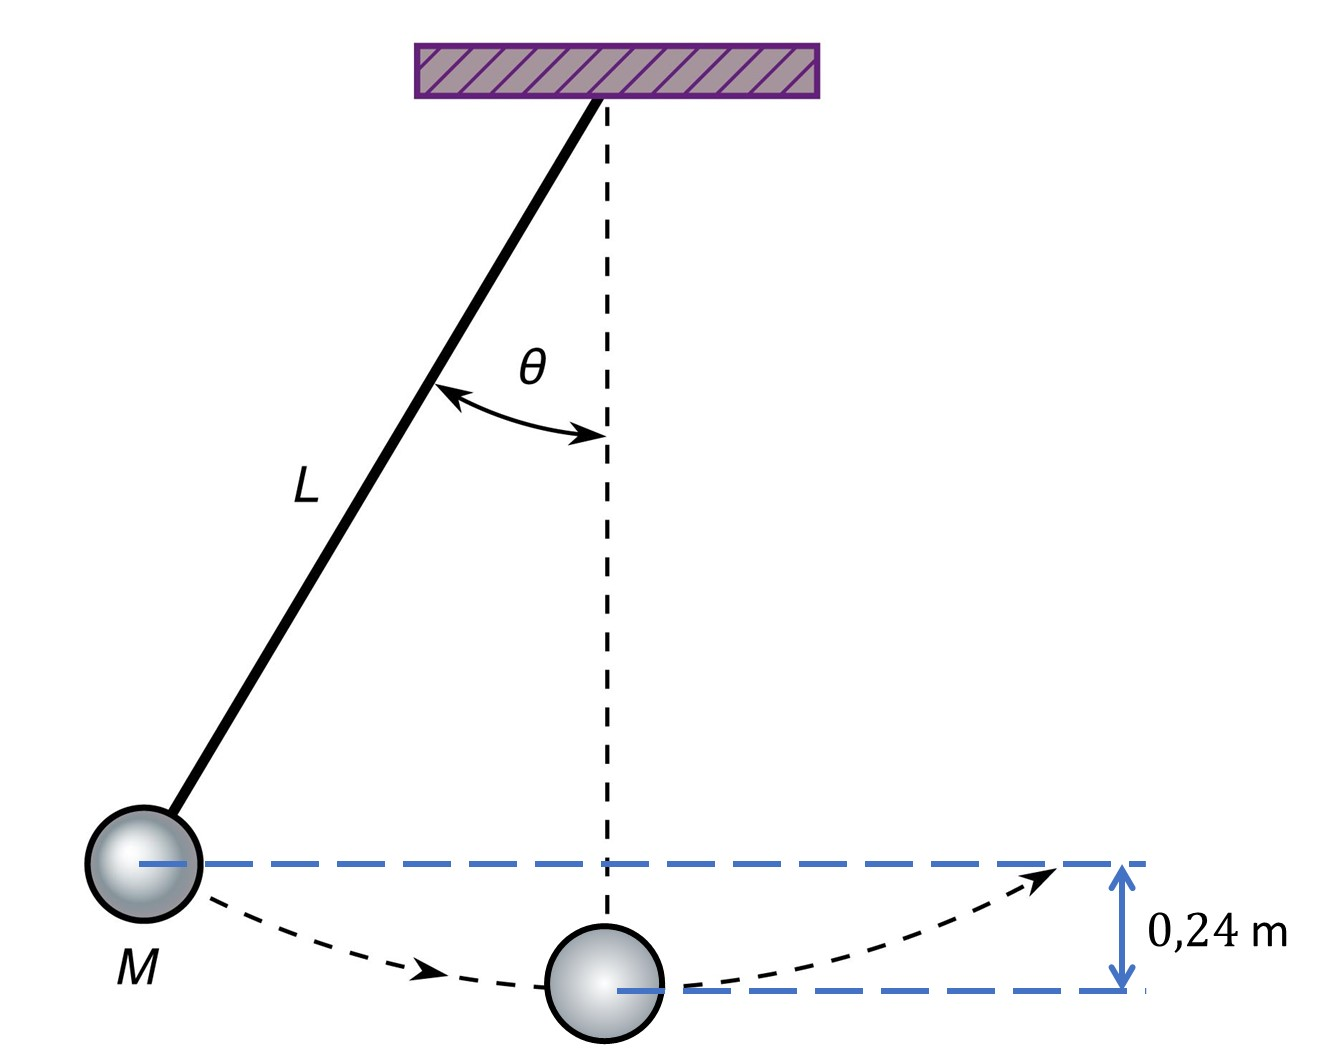
\includegraphics[scale=0.3]{../figs/D10-GK-HK2-2}}	
	\loigiai{}
\end{ex}
\Closesolutionfile{ans}
\section{Tự luận} 
\setcounter{ex}{0}
\Opensolutionfile{ans}[ans/D10-GK-HK2-001-TL]
% ===============================================================
\begin{ex}
	Cây đàn piano có trọng lượng $\SI{3.5}{\kilo\newton}$ được nâng lên với vận tốc không đổi lên một căn hộ cao $\SI{25}{\meter}$ so với mặt đường bằng một hệ thống ròng rọc gắn vào mái tòa nhà. Mỗi công nhân có thể cung cấp $\SI{165}{\watt}$ công suất và hệ thống ròng rọc có hiệu suất \SI{75}{\percent}. Bỏ qua khối lượng của ròng rọc, thời gian cần thiết để 1 người công nhân có thể nâng cây đàn từ mặt đường lên căn hộ là bao nhiêu giây? \textit{(Kết quả làm tròn đến chữ số hàng đơn vị)}.
	\loigiai{
		$W=Ph=\SI{87500}{\joule}$\\
		$t=\dfrac{W}{\eta P_{total}}=\SI{707}{\second}$.
	}
\end{ex}
% ===============================================================
\begin{ex}
	Một vật khối lượng $m=\SI{100}{\gram}$ được thả rơi tự do từ độ cao $H=\SI{20.0}{\meter}$ so với mặt đất (được chọn làm mốc thế năng). Biết gia tốc rơi tự do $g=\SI{9.80}{\meter/\second^2}$.
	\begin{enumerate}[label=\alph*)]
		\item Tính cơ năng của vật.
		\item Tính độ lớn vận tốc tiếp đất của vật.
		\item Khi động năng của vật gấp ba lần thế năng của nó thì vật cách mặt đất một khoảng bằng bao nhiêu?
	\end{enumerate}
	\loigiai{
		\begin{enumerate}[label=\alph*)]
			\item $W=\SI{19.6}{\joule}$.
			\item $v_{\text{cđ}}=\sqrt{2gH}\approx\SI{19.8}{\meter/\second}$.
			\item $h=\dfrac{1}{4}H=\SI{5}{\meter}$.
		\end{enumerate}
	}
\end{ex}
% ===============================================================
\begin{ex}
	Một viên đạn \SI{30}{\gram} đang bay ngang với tốc độ \SI{500}{\meter/\second} thì đâm xuyên \SI{12}{\centi\meter} vào một bức tường rắn rồi dừng lại.
	\begin{enumerate}[label=\alph*)]
		\item Tìm độ giảm cơ năng của viên đạn.
		\item  Giả sử lực do bức tường tác dụng lên đạn là không đổi. Hãy tìm độ lớn của lực này.
	\end{enumerate}
	\loigiai{
		\begin{enumerate}[label=\alph*)]
			\item $W_1-W_2=\SI{3750}{\joule}$.
			\item $F_c=\SI{31250}{\newton}$.
		\end{enumerate}
	}
\end{ex}
\Closesolutionfile{ans}
\begin{center}
	\textbf{--- HẾT ---}
\end{center}